\documentclass[12pt]{article}
\usepackage{xeCJK}%preamble part
\usepackage{graphicx}
\usepackage{indentfirst}
\usepackage[a4paper, inner=1.5cm, outer=3cm, top=2cm, bottom=3cm, bindingoffset=1cm]{geometry}
\usepackage{epstopdf}
\usepackage{listings}
\usepackage{array}
\usepackage{fontspec}
\usepackage{gensymb}
\usepackage{todonotes}
\usepackage{amsmath}
\usepackage[citecolor=blue]{hyperref}

\usepackage{makecell}
\usepackage[lofdepth,lotdepth]{subfig}




\setlength{\extrarowheight}{4pt}
\setlength{\parindent}{1cm}
\begin{document}
\title{\textbf{\fontsize{15.75pt}{\baselineskip}{讨论}}} 

\author{\fontsize{12pt}{\baselineskip}{数33 赵丰}}
\maketitle
\large
在协作定位网络中,节点位置先验分布的误差和定位过程中产生的误差会在网络节点中传播。
关于协作定位分层的再讨论:
在杨思怡的毕设论文中是把目标节点放在重排后FIM的左上角,这样计算
J(k)就含有k层递归式子,处理起来非常不方便。为此可以考虑把她的
FIM镜像一下,让目标节点在FIM右下角,这样EFIM是求最
右下角的那个。
沿用之前提到的Chlosky Decomposition的思路,设FIM=$LL^T$,其中
L是下三角阵,则$FIM^{-1}=L^{-T}L^{-1}$,注意$=L^{-T}$是上三角阵,
$L^{-1}$是下三角阵,$FIM^{-1}$的右下角元素是$L^{-1}$右下角元素的平方。而由Gaussian Elimination方法可知$L^{-1}$右下角元素等于
L右下角元素的倒数,因此只需研究L右下角元素的结构性质。实际上
从杨思怡的定理2.4也可以看出,里面的矩阵是有对称性的,最中间的
那个可以分解成$L_1L_1^T$的形式后最终$J(k)$也能写成$L_2L_2^T$的形式,直接考虑整体会很大程度上增加矩阵运算的难度,所以应该可以只考虑一半降低难度。
下面先以$V_0,V_1,V_2$三层节点为例说明这个问题:
\begin{figure}[!ht]
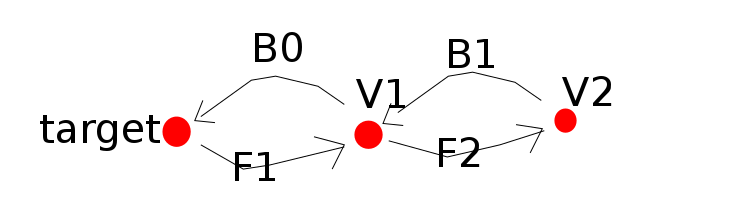
\includegraphics[width=\linewidth]{001.png}
\end{figure}

在只有一个目标节点$V_0$时,定位信息只能依靠它和锚点的通信得到,此时
$J_e(P,0)=\Sigma_0$.当有两个移动节点时,目标节点的定位信息增加了
来自V1的后向信息B0,而V1的定位既有来自锚点的定位信息$\Sigma_1$,又有来自V0的前向信息F1,故此时FIM镜像以后有如下形式
\[
\left(
\begin{array}{ccc}
\Sigma_2+F_2F_2^H & -F_2B_1^H & 0\\
-B_1F_2^H & \Sigma_1+F_1F_1^H+B_1B_1^H & -F_1B_0^H\\
0 & -B_0F_1^H & \Sigma_0+B_0B_0^H 
\end{array}
\right)
\]
为简便,先讨论:
\[
\left(
\begin{array}{ccc}
A_1 & D_1 & 0 \\
D_1^T & A_2 & D_2 \\
0 & D_2^T & A_3
\end{array}
\right)
\]
$A_1,A_2,A_3$是对称矩阵,上面各个分块的维数不一定相等。
可以直接验证这个矩阵可以写成$LL^T$的形式,
\begin{equation}
L=\left(
\begin{array}{ccc}
A_1^{\frac{1}{2}} & 0 & 0 \\
D_1^TA_1^{-\frac{1}{2}} & (A_2-D_1^TA_1^{-1}D_1)^{\frac{1}{2}} & 0 \\
0 & D_2^TL_{2,2}^{-1} & (A_3-D_2^TL_{2,2}^{-2}D_2)^{\frac{1}{2}}
\end{array}
\right)
\end{equation}
这个分解可以看成是FIM合同变换到单位矩阵的过程。通过初等合同变换
可以很容易看出这一点。
注意到迭代的中间步骤产生的$L_{2,2}^{-2}$,即第二行第二列元素的特征,
它是只考虑前两层节点时候的EFIM(不考虑开平方),如果只考虑对角线的
元素,三对角的Chlosky分解给出了计算前k层节点对目标节点信息量的计算清晰的迭代过程,如果考虑次对角线,可以看成第k层节点的信息$A_1$沿着楼梯形的路径传播到目标节点,即先与第k-1层节点耦合$L_{1,2}$,再对
第k-1层节点确定自身位置产生贡献$L_{2,2}$,然后信息从第k-1层节点
往里再传。

%胡乱看的:
%\url{https://en.wikipedia.org/wiki/Interval\_propagation}
%Interval Propagation方法,
%假设$x_1,x_2,...x_n$的初始估计区间分别为$I_1,I_2,...I_n$,
%$x_1,...x_n$满足一些等式或不等式约束,则Interval Propagation %Method可以根据初始的估计区间和约束条件计算后验的区间$I'
%_1,I'_2,...I'_n$使得$I'_i\subset I_i$
\end{document}